\subsection{Capacitors, Inductors, and AC circuits} 

%\DTMnewdatestyle{dateupdated}{〈definition 〉

Answers to M\Alph{subsection} problems are on page \pageref{C_L_and_AC_prob_answers}.  \textbf{\textcolor{red}{Updated \DTMnow.}}

%--------------------------------------------------------------------------------------------------------------
\begin{Exercise}
A 200 nF capacitor is charged by a 5~V supply through a $2\kohm$ resistor, starting at zero volts.  (a)~Graph both the current $I_C$ through the capacitor and the voltage $V_C$ across the capacitor as functions of time.  (b)~At what time does the capacitor voltage reach 90\% of the supply voltage?  (c)~What is the current through the resistor at the time you calculated in part (b)?
\end{Exercise}
\begin{Answer}
(b) $921~\mu$sec (c) $250~\mu$A
\end{Answer}

%--------------------------------------------------------------------------------------------------------------
\begin{minipage}{0.7\textwidth}
\begin{Exercise}
A student wants to find the internal resistance of a standard, size-AA battery.  With no load resistor connected, the voltage across the terminals of the battery is 1.55~V.  But when the battery is connected to a load resistor of 10~$\Omega$ (as shown on the right) the voltage across the load resistor is 1.47~V.  What is the internal resistance of the battery?
\end{Exercise}
\begin{Answer}
0.544~$\Omega$ The circuit is built correctly and the output is within the range expected for the tolerances of the components. The circuit is built correctly and the output is within the range expected for the tolerances of the components. The circuit is built correctly and the output is within the range expected for the tolerances of the components.
\end{Answer}
\end{minipage}
\begin{minipage}{0.30\textwidth - 5pt}
\hfill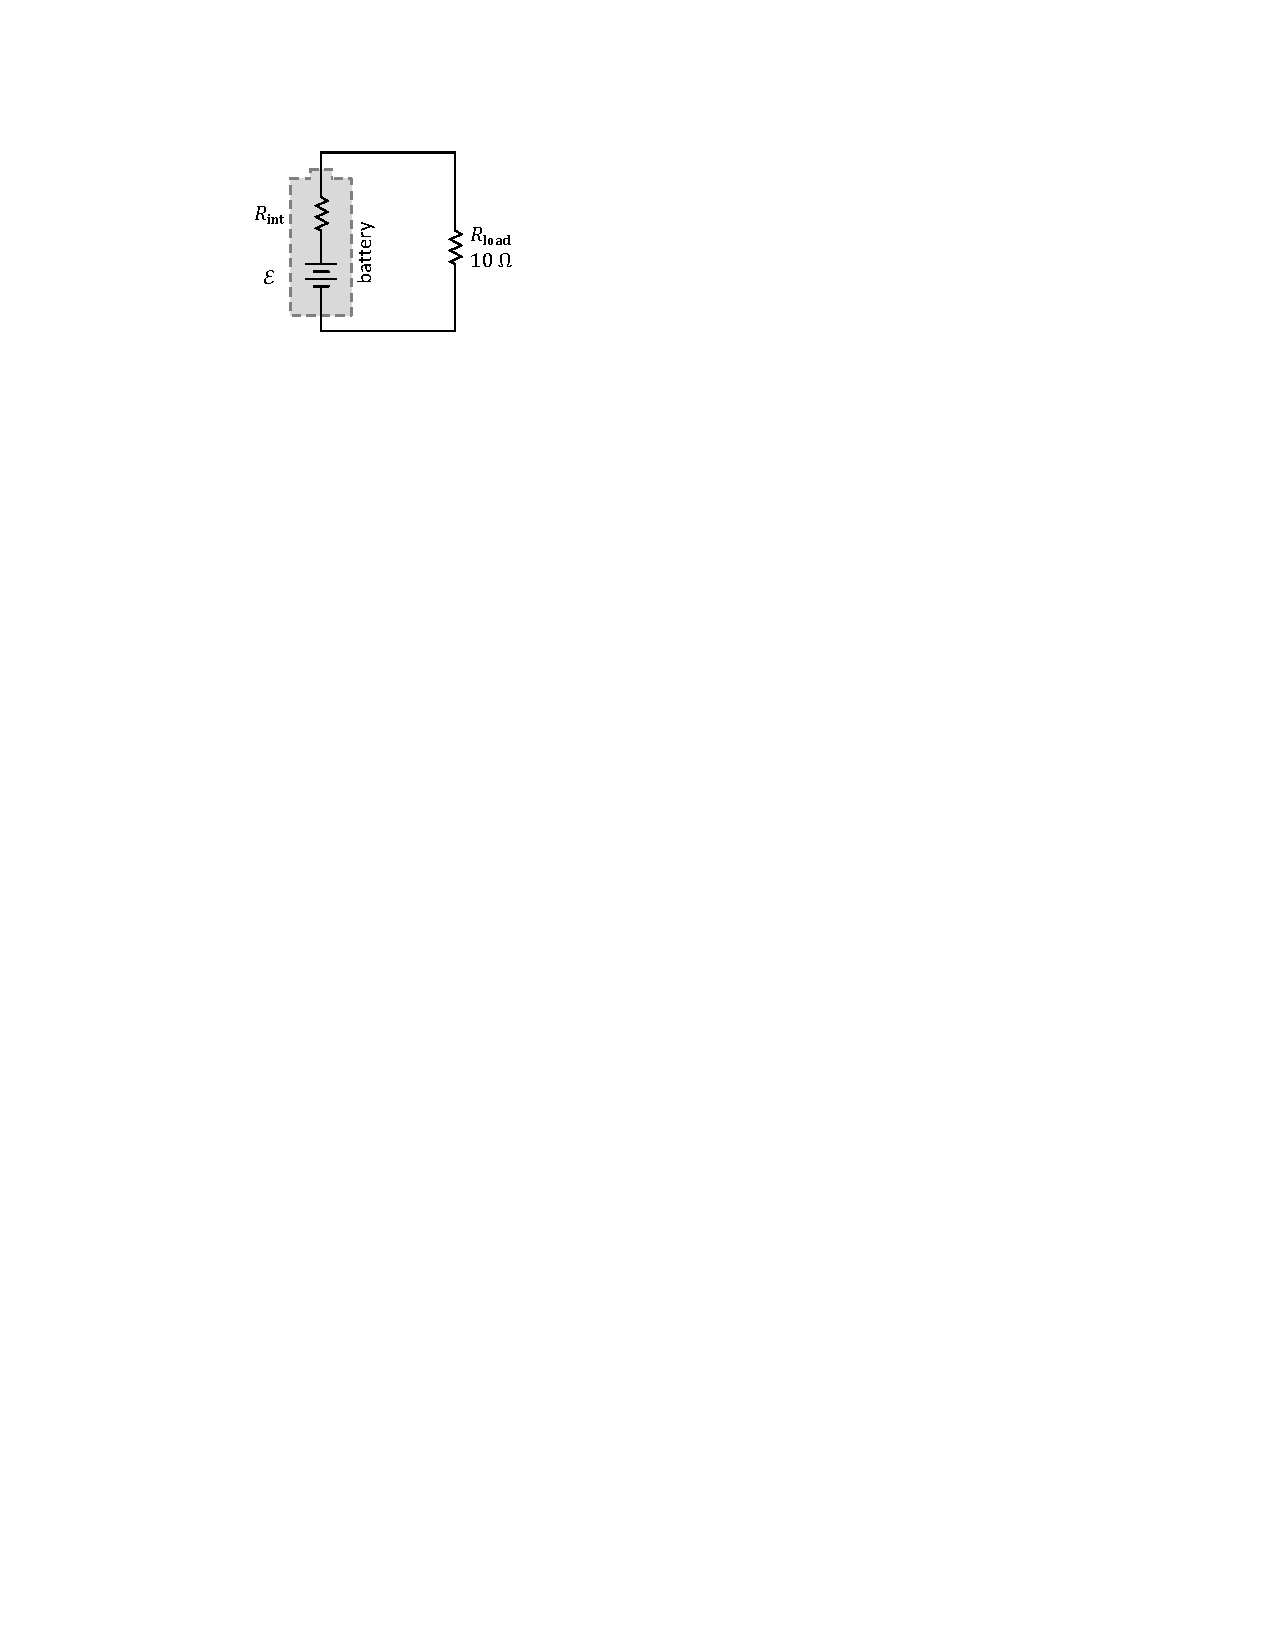
\includegraphics{M_problems/the_basics/real_battery_10ohms.pdf}
\end{minipage}

%--------------------------------------------------------------------------------------------------------------
\begin{Exercise}
The figures below show two possible circuits you could use to measure the current and voltage of a resistor.  Both methods are imperfect, due to the non-ideal input impedances of the voltmeter and the ammeter.  
(a)~Which circuit will give a current reading that is slightly inaccurate, due to the non-ideal voltmeter?  
(b)~Will that current reading be too high or too low?  
(c)~Which circuit will give a voltage reading that is slightly inaccurate, due to the non-ideal ammeter?  
(d)~Will that voltage reading be too high or too low? 
(e)~Suppose the impedances of the two meters are $10\ohm$ and $10\Mohm$.  Which circuit is preferable if the resistor you are measuring has $R=100\ohm$, and why?  (f) Which circuit is preferable if the resistor you are measuring has $R=1\Mohm$, and why?
\begin{center}
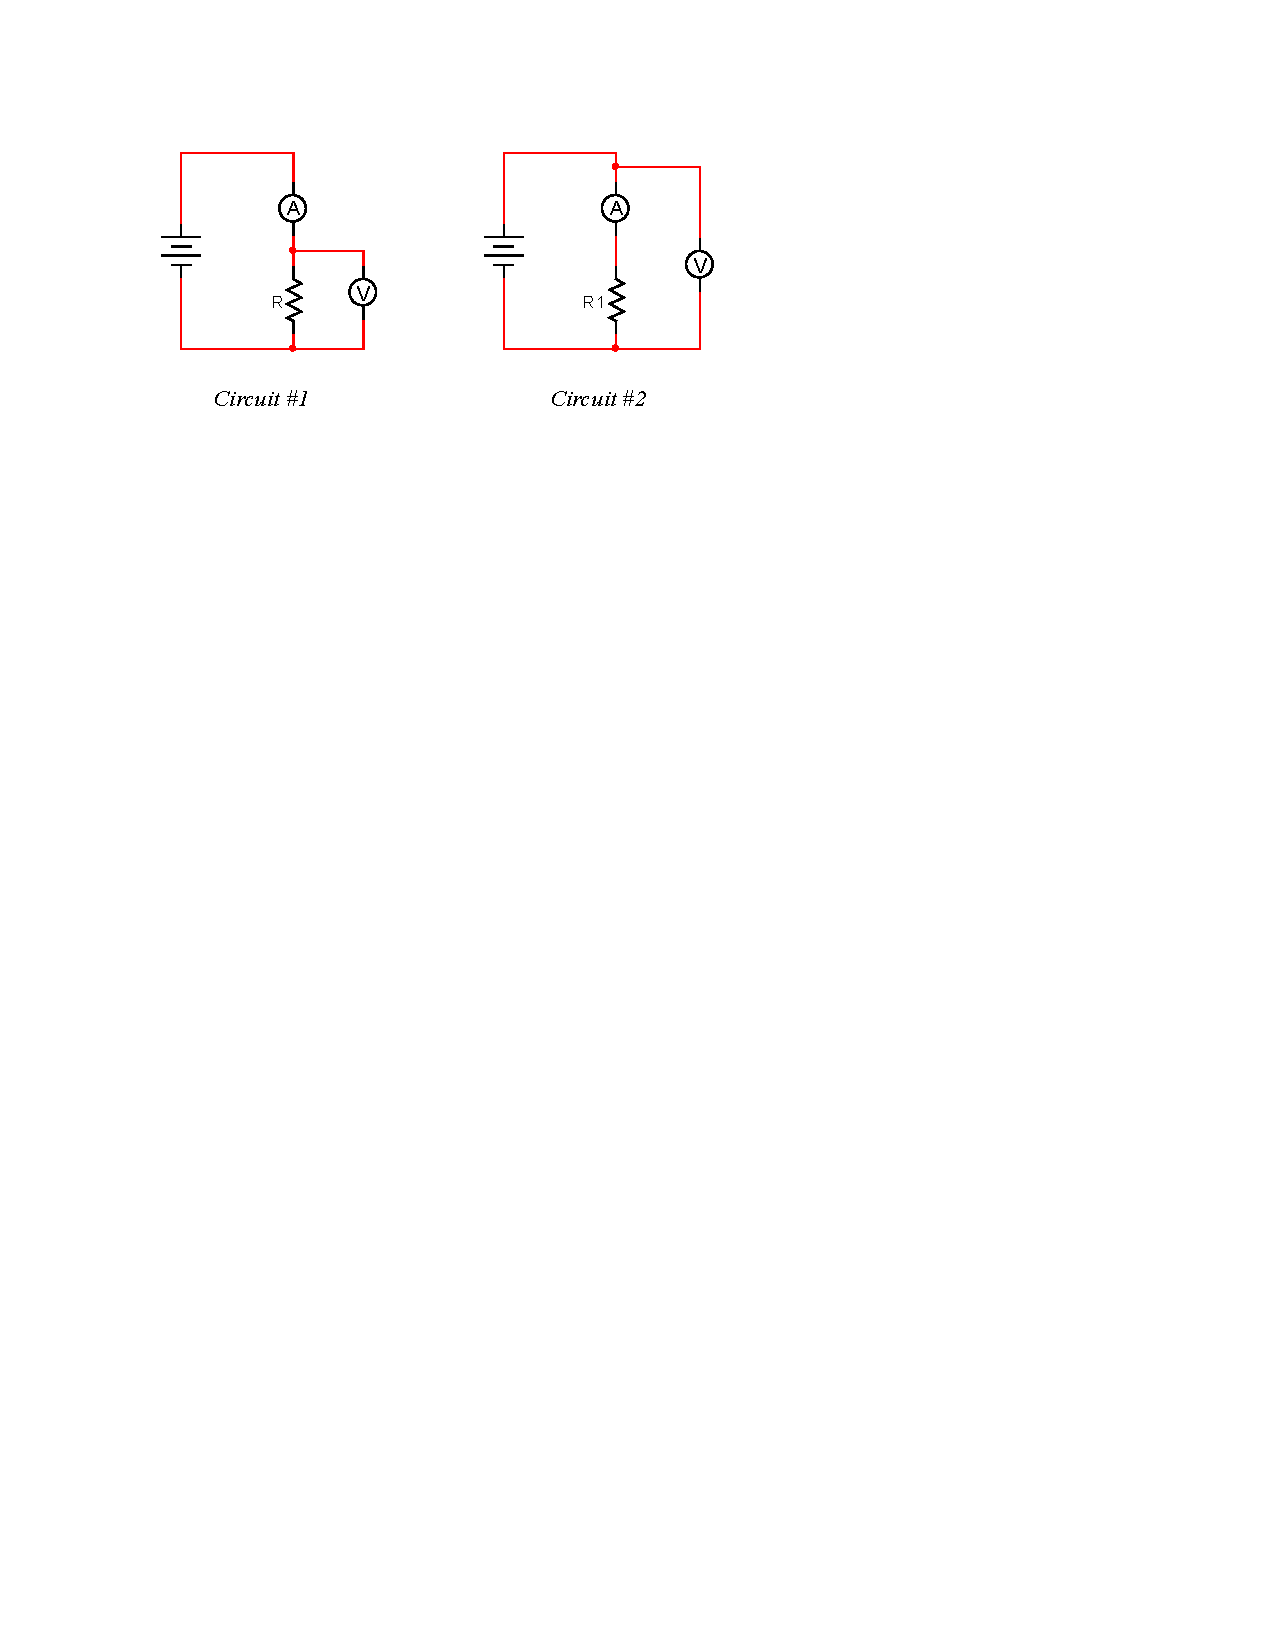
\includegraphics{M_problems/the_basics/I_V_measurements.pdf}
\index{color page}
\end{center}
\end{Exercise}
\begin{Answer}
(a) circuit \#1 (c) circuit \#2 (d) too high (e) circuit \#1
\end{Answer}

%\newcommand{\figuretoright}{3} {%
	%#1 is the picture width
	%#2 is the text to the right



%Ideas for additional problems:

%\vfill
%\pagebreak[3]

\vspace{0.7in}

\textbf{Answers to Selected {\thesubsection} Problems:}
\label{C_L_and_AC_prob_answers}
%\shipoutExercise
\shipoutAnswer

\cleardoublepage
